%%%%%%%%%%%%%%%%%%%%%%%%%%%%%%%%%%%%%%%%%%%%%%%%%%%%%%%%%%%%%%%%%%%%%%%%%%%%%%%
% Chapter 2 - Simultaneous Imaging of Cerebral Blood Flow and Oxygen Tension
%%%%%%%%%%%%%%%%%%%%%%%%%%%%%%%%%%%%%%%%%%%%%%%%%%%%%%%%%%%%%%%%%%%%%%%%%%%%%%%

\chapter{Simultaneous Imaging of Cerebral Blood Flow and Oxygen Tension} \label{ch:system}

Measurements of hemodynamic parameters in cerebral vasculature have been invaluable in preclinical research for understanding the physiology of the normal and diseased brain. The combination of imaging techniques to simultaneously measure multiple hemodynamic parameters has become increasingly common and used to study stroke \cite{Jones:2008gb}, cortical spreading depression \cite{Sakadzic:2009jo}, and functional brain activation \cite{Dunn:2005gw, Dunn:2003wy}. Advancements in computer processing power and the increased availability of lasers and light-emitting diodes across a diverse range of wavelengths have facilitated the development of these multi-parameter hemodynamic imaging platforms.

In 2010, Ponticorvo and Dunn \cite{Ponticorvo:2010uv} detailed a dual-modality imaging system capable of simultaneously measuring cerebral blood flow (CBF) and oxygen tension (\ce{pO2}) in cortical vasculature. The system combined laser speckle contrast imaging (LSCI) and oxygen-dependent quenching of phosphorescence. An unpublished modification to the system added multispectral reflectance imaging for measurements of oxy- and deoxyhemoglobin \cite{Ponticorvo:2010ur}. The primary innovation of this design was the use of a digital micromirror device (DMD) to achieve spatial localization of the phosphorescent signal. A DMD is an optical semiconductor device that consists of a two-dimensional array of thousands of individually addressable mirrors that can be tilted to spatially modulate light. By patterning excitation light, phosphorescence could be constrained to only the targeted regions of interest, which allowed the use of high sensitivity point detectors. This overcame the traditional limitations of spatially-resolved phosphorescence imaging that either required the use of expensive laser scanning systems \cite{Yaseen:2009ep, Kazmi:2013ey} or exposure-gated cameras \cite{Shonat:2003ia, Sakadzic:2009jo}.

However, a major limitation of this system was the phosphorescent probe Oxyphor R2 \cite{Dunphy:2002tz}, which required conjugation with albumin in order to remain stable \textit{in vivo}. The system was also optically limited to only targeting large regions of the field of view (FOV) for \ce{pO2} measurements and was incapable of performing multiple actions simultaneously with the DMD. This chapter details a redesign of the system by Ponticorvo and Dunn \cite{Ponticorvo:2010uv} with the goal of improving the spatial and temporal resolutions of both imaging modalities through implementation of newer hardware and a more robust oxygen-sensitive phosphorescent probe. The new imaging system was described in a methods paper published in \textit{Neurophotonics} \cite{Sullender:2018ff}.



%%%%%%%%%%%%%%%%%%%%%%%%%%%%%%%%%%%%%%%%%%%%%%%%%%%%%%%%%%%%%%%%%%%%%%%%%%%%%%%
% Section 2.1 - Instrumentation
%%%%%%%%%%%%%%%%%%%%%%%%%%%%%%%%%%%%%%%%%%%%%%%%%%%%%%%%%%%%%%%%%%%%%%%%%%%%%%%
\section{Instrumentation}

The following dual-modality imaging system combines LSCI with oxygen-dependent quenching of phosphorescence for the simultaneous measurement of CBF and \ce{pO2}. Because LSCI is rarely light-limited, the optical design is focused on the projection of patterned excitation light off the DMD and the efficient collection of the emitted phosphorescence. The spectral cutoffs for the system were dictated by the new phosphorescent probe, Oxyphor PtG4 \cite{Esipova:2011hi}, an oxygen-sensitive dendritic probe that contains Platinum(II)-\textit{meso}-tetra-(3,5-dicarboxyphenyl)tetrabenzoporphyrin (PtTBP) as the phosphorescent core.

% Figure - Oxyphor PtG4 Spectra + Calibration
\begin{figure}
    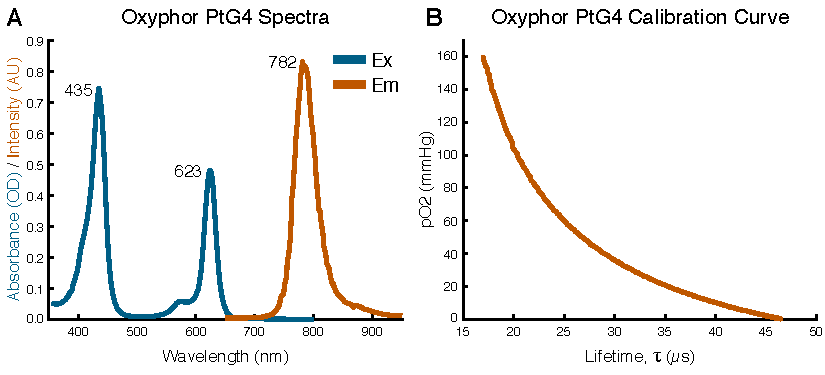
\includegraphics{figures/chapter_2/oxyphorptg4.pdf}
    \caption{
        \label{fig:oxyphor_ptg4}
        \textbf{(A)} Excitation (blue) and emission (red) spectra for Oxyphor PtG4. \textbf{(B)} Calibration curve relating environmental \ce{pO2} to the measured phosphorescence lifetime ($\tau$) under physiological conditions (37 $^\circ$C, pH 7.2).
    }
\end{figure}

Unlike its predecessors Oxyphor R2 and G2 \cite{Dunphy:2002tz}, which were limited to albumin-rich environments for stability, Oxyphor PtG4 is encapsulated within a hydrophobic dendrimer and PEGylated to increase solubility and biocompatibility. These modifications provide increased stability across a wider range of temperatures and pH values and eliminate the need for conjugation with blood proteins \cite{Esipova:2011hi}. Oxyphor PtG4 has two excitation maxima near 435 nm (Soret) and 623 nm (Q band) and a broad emission spectra peaking at 782 nm (Figure \ref{fig:oxyphor_ptg4}A). The probe was calibrated under physiological conditions (37 $^\circ$C, pH 7.2) by measuring the phosphorescent decay lifetime ($\tau$) as the environmental \ce{pO2} was increased from 0 mmHg to 160 mmHg (Figure \ref{fig:oxyphor_ptg4}B). The unquenched lifetime ($\tau_0$) is 47 $\mu$s in an oxygen-free environment.

%%%%%%%%%%%%%%%%%%%%%%%%%%%%%%%%%%%%%%%%%%%%%%%%%%%%%%%%%%%%%%%%%%%%%%%%%%%%%%%
\subsection{Optical System}

The schematic of the optical system can be seen in Figure \ref{fig:systemschematic_1}. The excitation and emission spectra of Oxyphor PtG4 dictated laser selection and dichroic beamsplitter cutoff wavelengths. LSCI was performed using a 685 nm laser diode (50 mW, HL6750MG, Thorlabs, Inc.) illuminating the sample at an oblique angle. The laser was mounted in a temperature-controlled housing (TCLDM9, Thorlabs, Inc.) and collimated with a slight divergence using an aspheric lens (C240TME-B, Thorlabs, Inc.) to illuminate the entire FOV. The operating current was set using a laser diode controller (LDC202, Thorlabs, Inc.) and the diode temperature regulated using a temperature controller (TED200C, Thorlabs, Inc.). The scattered light was relayed through a pair of dichroic beamsplitters and a bandpass filter (685$\pm$40 nm, S685/40m, Chroma Technology Corp.) to an NIR-enhanced CMOS camera (acA1300-60gmNIR, 1280 x 1024 pixels, Basler AG) with 2x magnification for a FOV of 3.5 x 2.8 mm. The camera was controlled via the Basler Pylon API using custom software written in C++ (i.e. the ``Speckle Software'').

% Figure - System Schematic (Ver. 1)
\begin{figure}
    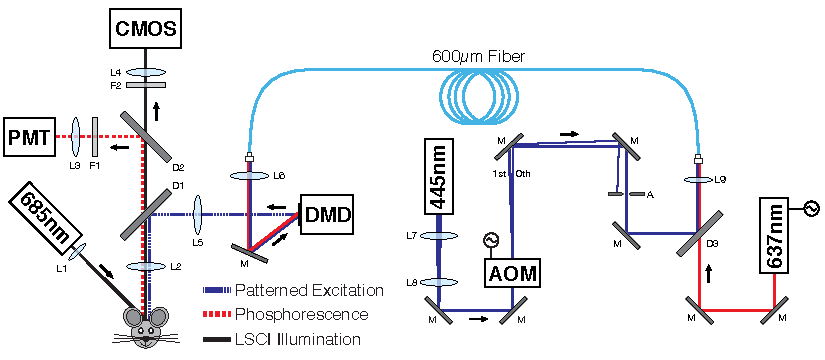
\includegraphics{figures/chapter_2/systemschematic.pdf}
    \caption{
        \label{fig:systemschematic_1}
        Schematic of the dual-modality imaging system combining LSCI with oxygen-dependent quenching of phosphorescence.
    }
\end{figure}

Separately, two different lasers at 445 nm and 637 nm were selected to target the Soret and Q band excitation maxima of Oxyphor PtG4. Each laser can be used independently to collect phosphorescence lifetime measurements with different penetration depths and sample volumes because of their wavelengths. The 445 nm laser (200 mW, AixiZ) is a packaged device with a 4 mm collimated output that operates at a fixed current with convection cooling. The beam size was reduced to 1 mm and gated using an 80 MHz acousto-optic modulator (23080-2-LTD AOM and 21080-1AM RF Driver, Neos Technologies, Inc.). The 637 nm laser diode (250 mW, HL6388MG, Thorlabs, Inc.) was mounted in a temperature-controlled housing (LDM21, Thorlabs, Inc.) and collimated using an aspheric lens (C330TME-B, Thorlabs, Inc.). The laser was directly gated using its driver (LDD400-1P, Wavelength Electronics, Inc.) and the diode temperature regulated using an external temperature controller (300B, Newport Corp.). Both lasers were gated via analog modulation to produce 20 $\mu$s pulses of light for time domain lifetime measurements.

The lasers were coaligned using a red hot mirror (580 nm cutoff, FM02, Thorlabs, Inc.) and coupled into a fiber optic patch cord (P600-2-VIS-NIR, Ocean Optics, Inc.) with a 600 $\mu$m core size. The modulated laser light was relayed to the primary imaging system via the patch cord and re-collimated to illuminate the DMD. A DLP LightCrafter Evaluation Module (Texas Instruments) was modified to expose the bare DMD (DLP3000, 608 x 684 pixels, 7.6 $\mu$m pitch, Texas Instruments) for illumination. The spatially patterned modulated light was then relayed to the sample with 0.5x magnification to selectively excite Oxyphor PtG4 for lifetime measurements.

The emitted phosphorescence was separated from the excitation and scattered LSCI laser light using a pair of dichroic beamsplitters (650 nm, ZT640rdc, Chroma Technology and 750 nm, FF750-SDi02, Semrock, Inc.) and a bandpass filter (810$\pm$90 nm, ET810/90m, Chroma Technology Corp.) and relayed to a photomultiplier tube for detection (H7422P-50, Hamamatsu Photonics K.K.). Figure \ref{fig:systemspectra} contains an overview of the spectral separation in the imaging system and Table \ref{tab:filters} details each filter in the primary imaging path.

% Figure - System Spectra
\begin{figure}
    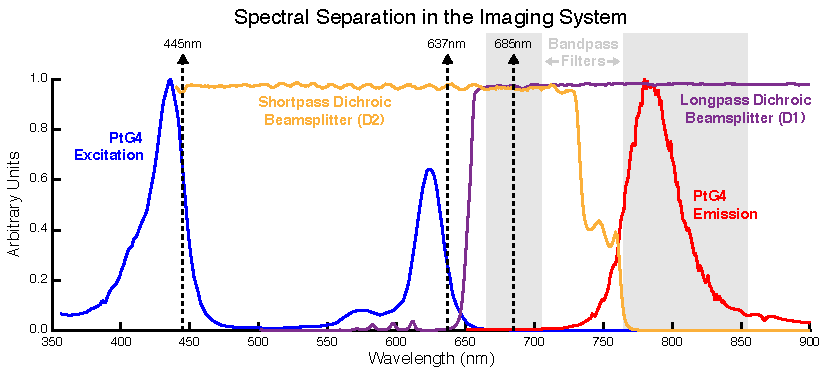
\includegraphics{figures/chapter_2/systemspectra.pdf}
    \caption{
        \label{fig:systemspectra}
        Dichroic beamsplitters and bandpass filters used to spectrally separate light in the imaging system. A longpass dichroic beamsplitter (purple) separates the excitation lasers (445 and 637 nm) from the scattered LSCI laser (685 nm) and Oxyphor PtG4 phosphorescence emission (red). A shortpass dichroic beamsplitter (gold) separates the LSCI light from the phosphorescence for detection. Bandpass filters (shaded grey) limit ambient and scattered light from reaching the detectors. All values are normalized.
    }
\end{figure}

% Table - Filter Summary
\begin{table}
    \caption{Summary of optical filters in the imaging system}
    \label{tab:filters}
    \centering
    \resizebox{\textwidth}{!}{
    \begin{tabular}{ccccc} \addlinespace \toprule
        \thead{Label} & \thead{Filter} & \thead{Usage} & \thead{Manufacturer} & \thead{Part Number} \\ \midrule
        \textbf{D1} & \makecell{650 nm longpass \\ dichroic beamsplitter} & \makecell{Excitation \\ Separation} & Chroma & ZT640rdc \\ \hline
        \textbf{D2} & \makecell{750 nm shortpass \\ dichroic beamsplitter} & \makecell{Emission \\ Separation} & Semrock & FF750-SDi02-25x36 \\ \hline
        \textbf{D3} & \makecell{580 nm red hot mirror} & \makecell{Laser \\ Coalignment} & Thorlabs & FM02 \\ \hline
        \textbf{F1} & \makecell{810$\pm$90 nm \\ bandpass} & \makecell{Phosphorescence \\ Isolation} & Chroma & ET810/90m \\ \hline
        \textbf{F2} & \makecell{685$\pm$40 nm \\ bandpass} & \makecell{LSCI \\ Isolation} & Chroma & S685/40m \\ \bottomrule
    \end{tabular}}
\end{table}

%%%%%%%%%%%%%%%%%%%%%%%%%%%%%%%%%%%%%%%%%%%%%%%%%%%%%%%%%%%%%%%%%%%%%%%%%%%%%%%
\subsection{Acquisition Control} \label{ssec:acquisition_control}

An overview of the control system can be seen in Figure \ref{fig:controlschematic}. Both LSCI and the phosphorescence lifetime measurements were performed simultaneously using a single computer. The LSCI acquisition is controlled via the Speckle Software, which implements the Basler Pylon API for comprehensive control of the GigE camera. The Speckle Software allows for the real-time calculation, display, and writing of speckle contrast imagery using an efficient processing algorithm \cite{Tom:2008tg}. The camera was operated with a 5 ms exposure time, which is standard for \textit{in vivo} microvasculature studies using LSCI \cite{Yuan:2005tj}. Raw intensity images were acquired in bursts and saved at an effective 60 frames per second (fps) at an 8-bit bit depth. The computed speckle contrast images were saved as single-precision floating-point numbers and averaged together ($n$ = 45 frames) during post-processing for a final frame rate of 1.33 fps. A standard LSCI acquisition produced data at a rate of 55 MB/s.

% Figure - System Control Schematic
\begin{figure}
    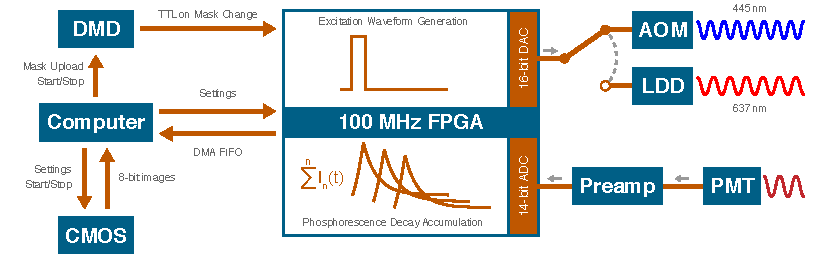
\includegraphics{figures/chapter_2/controlschematic.pdf}
    \caption{
        \label{fig:controlschematic}
        Imaging system control schematic. The phosphorescence excitation waveform can be sent to either the AOM for modulating the 445 nm laser or the LDD for modulation the 637 nm laser.
    }
\end{figure}

The Speckle Software was also modified to control the DMD via its Ethernet-over-USB command interface. Users can define arbitrarily-shaped regions of interest (ROIs) using the LSCI camera as reference and upload the resulting binary masks to the DMD for the patterning of excitation light. Registration between the camera and the projected pattern can be performed using the Speckle Software to guarantee alignment with the reference image (see Section \ref{ssec:dmd_registration}). Individual patterns or timed pattern sequences can be uploaded and displayed on the DMD, with a TTL pulse emitted on each pattern change.

While the Speckle Software controls the patterning of excitation light for the lifetime measurements, a separate LabVIEW (National Instruments Corp.) program controls the waveform generation and phosphorescence decay acquisition. A field-programmable gate array (FPGA) operating on a single-cycle timed loop oversees digital-to-analog (DAC) and analog-to-digital (ADC) conversion. The FlexRIO FPGA (PXIe-7965R, National Instruments Corp.) and 100 MHz transceiver module (NI-5781, National Instruments Corp.) reside in a PXI chassis (PXIe-1082, National Instruments Corp.) with a high-bandwidth embedded controller (PXIe-8130, National Instruments Corp.). The FPGA communicates with the host computer over a 1 Gigabit Ethernet connection.

Waveform generation and acquisition occur simultaneously on the FPGA with each complete cycle taking 32,768 ticks at the 100 MHz clock rate. Each cycle is triggered upon DMD pattern change via TTL through an auxiliary input on the transceiver. The excitation waveform contains a 20 $\mu$s square pulse (2,000 ticks) for an overall 6\% duty cycle and is output from the transceiver DAC between 0-1 V. Minimizing the pulse duration and duty cycle were important because high excitation flux levels can produce damaging levels of singlet oxygen \cite{Wilson:2005te}. If the 445 nm laser is being used, then the analog signal is directed into the AOM. If the 637 nm laser is being used, then the output is inverted and connected to the laser diode driver. The resulting phosphorescence is detected by the PMT and amplified at a fixed 50 mV/$\mu$A gain at 10 MHz (C9999, Hamamatsu Photonics K.K.). The analog signal is digitized by the transceiver ADC with a 14-bit depth resolution. In order to reduce the amount of data being saved, the FPGA accumulates the sum of $n$ cycles of phosphorescent decays before transferring to the host computer via a direct memory access (DMA) FIFO buffer. The LabVIEW program writes the accumulated phosphorescent signal to a binary file (32-bit integer) for post-processing. An optional setting enables on-the-fly fitting of the phosphorescence decay curve for $\tau$ and estimates the \ce{pO2} using the Oxyphor PtG4 calibration curve. However, this added computation can result in DMA FIFO overflow at higher acquisition speeds.

% Table - Lifetime Measurement Settings
\begin{table}
    \caption[Common phosphorescence lifetime acquisition settings]{
        Common acquisition settings for the phosphorescence lifetime measurements ($n$ = number of DMD patterns). Raw data is acquired by the FPGA at a rate of 160 MB/s.
    }
    \label{tab:lifetime_settings}
    \centering
    \resizebox{\textwidth}{!}{
    \begin{tabular}{cccc} \addlinespace \toprule
        \thead{\makecell{Pattern Rate \\ (Hz)}} & \thead{\makecell{Decays Accumulated \\ (per Pattern)}} & \thead{\makecell{Temporal \\ Resolution (s)}} & \thead{\makecell{Host Data \\ Rate (KB/s)}} \\ \midrule
        1 & 2500 & $n$ & 64 \\ \hline
        2 & 1250 & $n/2$ & 128 \\ \hline
        10 & 250 & $n/10$ & 640 \\ \hline
        50 & 50 & $n/50$ & 3200 \\ \hline
        100 & 25 & $n/100$ & 6400 \\ \bottomrule
    \end{tabular}}
\end{table}

Unlike LSCI, which operates at a fixed frame rate, the temporal resolution of the phosphorescence lifetime measurements is linearly dependent upon the number of patterns being displayed on the DMD and the number of decays accumulated on the FPGA. The digital controller on the DLP LightCrafter can store 96 binary patterns on its internal memory buffer and operate at a maximum pattern rate of 4000 Hz. The number of decays to accumulate on the FPGA is ultimately determined by the strength of the phosphorescent signal, which is influenced by the projected pattern size, Oxyphor PtG4 concentration, and laser power. The amount of data transferred to the host computer is inversely proportional to the number of records accumulated. Table \ref{tab:lifetime_settings} details several acquisition settings for the phosphorescence lifetime measurements with the 2 and 10 Hz pattern rates most commonly being utilized. While higher pattern rates offer higher temporal resolutions, the reduced averaging of the phosphorescent decays negatively affects the quality of the lifetime fitting.

A summary of the acquisition timing can be seen in Figure \ref{fig:timingschematic} with both LSCI and the phosphorescence lifetime measurements operating simultaneously but independently. This is possible because of the spectral separation of the excitation and emission wavelengths (Figure \ref{fig:systemspectra}). Both imaging modalities share the same computer clock, so timestamps can easily be aligned during post-processing.

% Figure - Acquisition Timing
\begin{figure}
    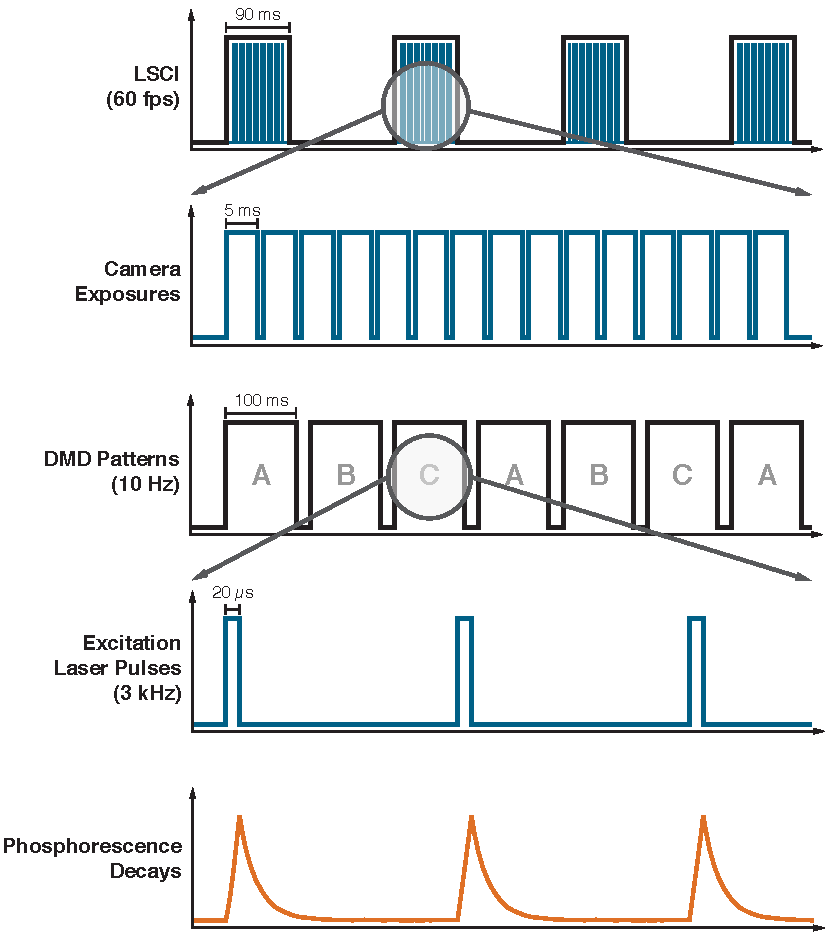
\includegraphics{figures/chapter_2/timingschematic.pdf}
    \caption{
        \label{fig:timingschematic}
        Acquisition timing paradigm for the LSCI and phosphorescence lifetime measurements.
    }
\end{figure}

%%%%%%%%%%%%%%%%%%%%%%%%%%%%%%%%%%%%%%%%%%%%%%%%%%%%%%%%%%%%%%%%%%%%%%%%%%%%%%%
\subsubsection{Troubleshooting}

During development of the phosphorescence lifetime measurement system, two significant problems were encountered. The first was a severe bandwidth limitation in the original preamplifier (SR570, Stanford Research Systems) used to convert the current output from the PMT to a voltage signal for ADC. The preamplifier was operated in “high bandwidth” mode with no filters active and a gain of 50 mV/$\mu$A. This corresponds to a bandwidth between 200-800 kHz. The maximum possible bandwidth is 1 MHz and can only be achieved at the lowest gain setting. This bandwidth is insufficient to properly sample the phosphorescent decay curve at higher \ce{pO2} levels as $\tau$ grows exponentially shorter (Figure \ref{fig:oxyphor_ptg4}B). The limitation was identified while performing measurements under ambient conditions where \ce{pO2} \textgreater 150 mmHg. At this \ce{pO2} level, a 1 $\mu$s change in $\tau$ corresponds to over a 20 mmHg change in \ce{pO2}. The problem was resolved by transitioning to the higher bandwidth (10 MHz) preamplifier detailed in Section \ref{ssec:acquisition_control}. The \textgreater 10x increase in bandwidth allows for proper sampling of the entire physiologically-relevant portion of the Oxyphor PtG4 calibration curve.

The second issue was related to the clock settings for the single-cycle timed loop on the FPGA. The PXIe-7965 FPGA module offers an onboard 40 MHz clock that was selected by default as the clock for the timed loop. However, this requires crossing clock domains from the 100 MHz sample clock on the NI-5781 transceiver to the onboard clock of the FPGA module. This can result in data corruption because the FPGA can capture data as it is actively being updated at the higher sample rate. In order to safely cross clock domains while guaranteeing data integrity, a FIFO buffer must be implemented. Alternatively, the sample clock on the transceiver module can be used as the clock for the single-cycle timed loop, which is how the issue was resolved on this system. Operating at 100 MHz does result in oversampling our expected signal, which is a problem that could be resolved by discarding unwanted samples.

%%%%%%%%%%%%%%%%%%%%%%%%%%%%%%%%%%%%%%%%%%%%%%%%%%%%%%%%%%%%%%%%%%%%%%%%%%%%%%%
\subsection{DMD Alignment} \label{ssec:dmd_registration}

Proper alignment and illumination of the DMD is critical for accurately projecting the excitation light patterns. The DLP3000 DMD contains a 0.3-inch diagonal micromirror array with 608 x 684 pixels arranged in a diamond configuration with a $\pm$12$^\circ$ tilt angle (Figure \ref{fig:dmdmirror}A). The DMD must be illuminated at -24$^\circ$ from the normal for the specularly reflected light from mirrors in the ON position to be directed along the desired optical axis (Figure \ref{fig:dmdmirror}B). Light reflected from pixels in the OFF position will be directed +48$^\circ$ off axis and can easily be blocked.

Because coherent light is being utilized, diffraction off the two-dimensional (2D) micromirror array must be considered. The physics are analogous to that of a 2D diffraction grating, except that two separate diffraction patterns will be formed, each influenced by the two possible mirror positions (Figure \ref{fig:dmdmirror}C). The position of the $(0,0)$ order and the intensity envelope follows the specular reflection off the tilted mirror as described above. However, all other orders are dependent upon incident angle, mirror pitch, mirror angle, and wavelength \cite{TexasInstruments:2009tr}. Isolating light from an single order at a specific wavelength requires adjusting the incident angle until the intensity envelope is aligned with the desired order. This will result in the outbound light no longer being normal to the face of the DMD, which can complicate downstream alignment. Alternatively, the diffracted light can be collimated and focused onto to the desired projection location using a pair of lenses. This effectively images the face of the DMD to the sample plane using the same alignment procedure as incoherent light.

% Figure - DMD Mirror Explanation
\begin{figure}
    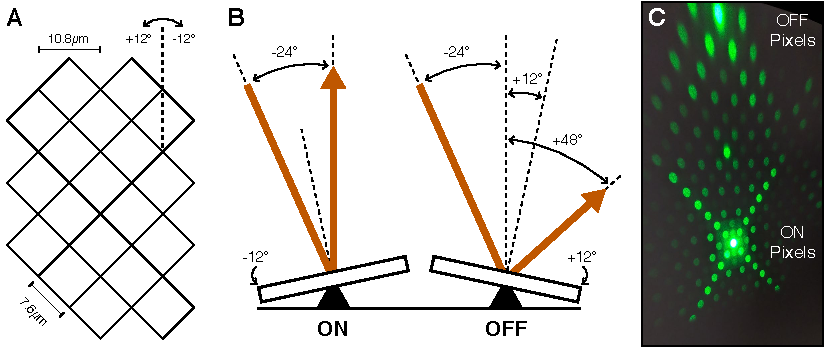
\includegraphics{figures/chapter_2/dmdmirror.pdf}
    \caption{
        \label{fig:dmdmirror}
        \textbf{(A)} Mirrors are arranged in a diamond configuration on the DMD with a 7.6 $\mu$m pitch and a $\pm$12$^\circ$ tilt angle. \textbf{(B)} Mirrors in the ON position will direct incident light perpendicular to the face of the DMD while mirrors in the OFF state will direct light off axis. \textbf{(C)} Diffraction patterns produced by coherent light illuminating the DMD.
    }
\end{figure}

% Figure - DMD Alignment
\begin{figure}
    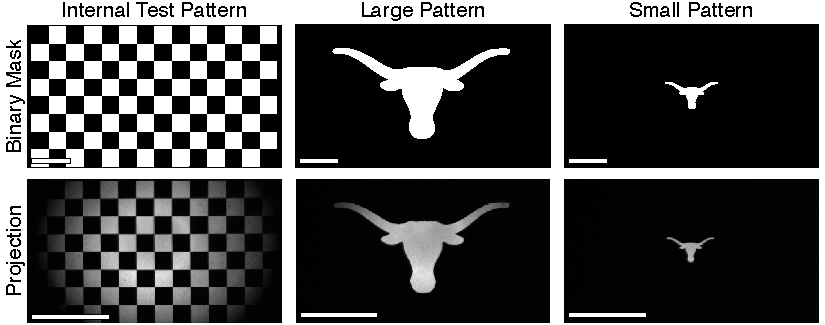
\includegraphics{figures/chapter_2/dmdalignment.pdf}
    \caption{
        \label{fig:dmdalignment}
        Test patterns used to perform and verify alignment of the DMD-projected light (Scale bars = 1 mm).
    }
\end{figure}

Alignment of the DMD was performed using a second camera (acA1300-60gmNIR, 1280 x 1024 pixels, Basler AG) placed at the focus of the objective lens to directly image the projected light. This was necessary because the two dichroic beamsplitters prevent excitation light from reaching the primary system camera. An internal checkerboard pattern on the DLP LightCrafter and external binary masks were used to verify that the diffraction orders were properly converging onto the sample plane (Figure \ref{fig:dmdalignment}). These images also verified the 0.5x optical magnification applied to the projected patterns. Because the DMD has a rectangular aspect ratio, the circular illuminating beam slightly underfills the active area, resulting in some peripheral mirrors being unusable for patterning. The Gaussian beam also produces a non-uniform intensity profile, which would be problematic for intensity-based imaging techniques but fortunately has minimal effect on lifetime measurements.

%%%%%%%%%%%%%%%%%%%%%%%%%%%%%%%%%%%%%%%%%%%%%%%%%%%%%%%%%%%%%%%%%%%%%%%%%%%%%%%
\subsection{DMD Registration} \label{ssec:dmd_registration}

In order to use the Speckle Software to define arbitrarily-shaped patterns, the camera FOV must be registered with the projection area of the DMD. An affine transform is used to translate, scale, shear, and rotate the mask from the camera coordinate system to the DMD coordinate system without linear distortion. The matrix representation of the 2D affine transform using homogeneous coordinates is defined as:
%
% Equation - Affine Transform
\begin{equation}
    \label{eq:affine}
    \begin{bmatrix}
        x' \\
        y' \\
        1  \\
    \end{bmatrix}
    =
    \begin{bmatrix}
        a & b & c \\
        d & e & f \\
        0 & 0 & 1 \\
    \end{bmatrix}
    \begin{bmatrix}
        x \\
        y \\
        1 \\
    \end{bmatrix}
\end{equation}
%
where $(x,y)$ represent camera coordinates and $(x',y')$ represent DMD coordinates. The Speckle Software performs the registration by prompting the user to identify the positions of three sequentially projected points in the camera FOV and then inverting Equation \ref{eq:affine} to solve for the six coefficients of the transformation matrix. While the dichroic beamsplitters limit the amount of excitation light that reaches the camera, the speckle contrast calculation is sensitive to the intensity changes when the bandpass filter is removed. The user can then define an ROI using the speckle contrast image for reference and the affine transform will be applied to the mask as it is uploaded to the DMD (Figure \ref{fig:dmdregistration}).

% Figure - DMD Registration
\begin{figure}
    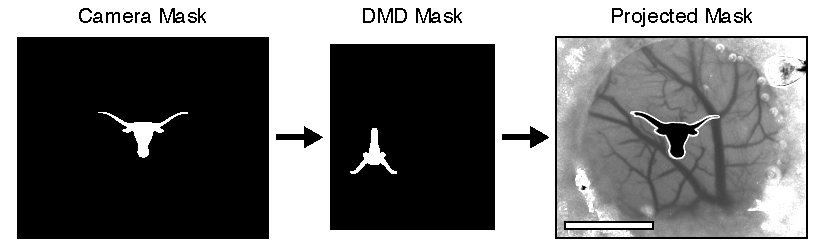
\includegraphics{figures/chapter_2/dmdregistration.pdf}
    \caption[Example of the affine image transformation applied to the camera coordinate space binary mask and the resulting DMD-projected pattern as imaged using LSCI.]{
        \label{fig:dmdregistration}
        Example of the affine image transformation applied to the camera coordinate space binary mask and the resulting DMD-projected pattern as imaged using LSCI (Scale bar = 1 mm). Adapted from \cite{Sullender:2018ff}.
    }
\end{figure}

%%%%%%%%%%%%%%%%%%%%%%%%%%%%%%%%%%%%%%%%%%%%%%%%%%%%%%%%%%%%%%%%%%%%%%%%%%%%%%%
\subsection{Laser Diode Stability} \label{ssec:laser_stability}

Laser diode stability is extremely important when performing LSCI because the technique is sensitive to changes in coherence and lasing wavelength. Regulated thermoelectric cooling (TEC) has been shown to significantly improve the stability of laser diode operation and reduce noise during LSCI measurements \cite{Richards:2016hy}. Identifying stable laser operating conditions requires adjusting the laser diode current and the TEC temperature setpoint. The 685 nm laser diode used for LSCI has a recommended operating current of 75 mA and exhibits temperature-dependent changes in slope efficiency and lasing wavelength.

The diode was tested under different operating conditions by imaging a static piece of paper and examining the stability of the intensity and speckle contrast over time within the center quadrant of the camera FOV (Figure \ref{fig:laserstability}A). A total of nine conditions were tested with laser diode currents varied between 65, 70, and 75 mA and TEC temperatures varied between 17, 18, and 19 $^\circ$C. The system was allowed to stabilize for five minutes after changing a parameter before acquiring LSCI data for ten minutes.

% Figure - Laser Diode Stability
\begin{figure}
    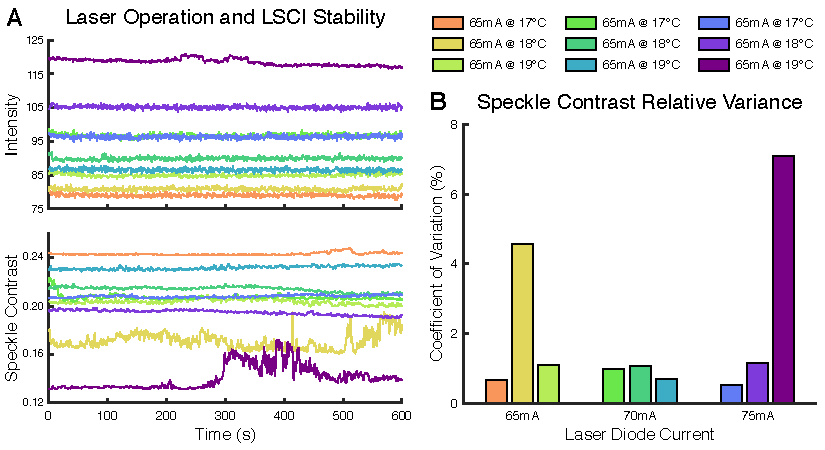
\includegraphics{figures/chapter_2/laserstability.pdf}
    \caption{
        \label{fig:laserstability}
        \textbf{(A)} Intensity and speckle contrast timecourses under different laser diode operating conditions. \textbf{(B)} Measurement of relative variance between the different speckle contrast data to identify the optimal laser diode operating conditions.
    }
\end{figure}

As expected, higher laser diode operating currents resulted in higher intensity values. With the exception of the 75 mA current at 19 $^\circ$C condition, minimal fluctuations in intensity were seen over time. However, the speckle contrast measurements exhibited much greater variation within and between acquisitions. Significant mode hopping, where the laser suddenly switches to a different resonator mode resulting in a discrete jump in the center wavelength, can be seen in both the 65 mA current at 18 $^\circ$C and 75 mA current at 19 $^\circ$C conditions. Mode hopping manifests in diode lasers because of temperature transients and non-ideal TEC operating temperatures. These fluctuations severely impact LSCI measurements and operating conditions must be optimized to mitigate them.

In order to identify the best operating parameters, the coefficient of variation (CV = $\sigma$ / $\mu$) for each speckle contrast timecourse was computed (Figure \ref{fig:laserstability}B). This statistic allows for the comparison of variation between data series with different means, with smaller values indicating less variance. Based on this metric, the 75 mA laser diode current at the 17 $^\circ$C TEC setpoint offered the best stability (CV = 0.05\%) for LSCI measurements. The stability of these settings were verified across two additional days of tests and were used exclusively throughout the remainder of this dissertation.



%%%%%%%%%%%%%%%%%%%%%%%%%%%%%%%%%%%%%%%%%%%%%%%%%%%%%%%%%%%%%%%%%%%%%%%%%%%%%%%
% Section 2.2 - Oxygen Tension Measurements in Cuvettes
%%%%%%%%%%%%%%%%%%%%%%%%%%%%%%%%%%%%%%%%%%%%%%%%%%%%%%%%%%%%%%%%%%%%%%%%%%%%%%%
\section{Oxygen Tension Measurements in Cuvettes}

Phosphorescence lifetime measurements were first tested in normoxic and anoxic cuvettes of 10 $\mu$M Oxyphor PtG4. The normoxic cuvette was prepared under ambient conditions and therefore has \ce{pO2} equivalent to that of air ($\sim$150 mmHg). The anoxic (0 mmHg) cuvette was created using the enzymatic reaction between glucose and glucose oxidase to scavenge oxygen from the sealed environment \cite{Lo:1997he}. Phosphorescent decays ($n$ = 200) were acquired using both 445 and 637 nm excitation with all DMD pixels in the ON position. The resulting decay curves were averaged and fitted for $\tau$ and the calibration curve used to lookup the corresponding \ce{pO2} value (Figure \ref{fig:cuvette}A). For both excitation wavelengths, the normoxic cuvette \ce{pO2} was 152 mmHg while the anoxic cuvette \ce{pO2} was 0 mmHg (Figure \ref{fig:cuvette}B).

% Figure - Cuvette pO2 Measurements
\begin{figure}
    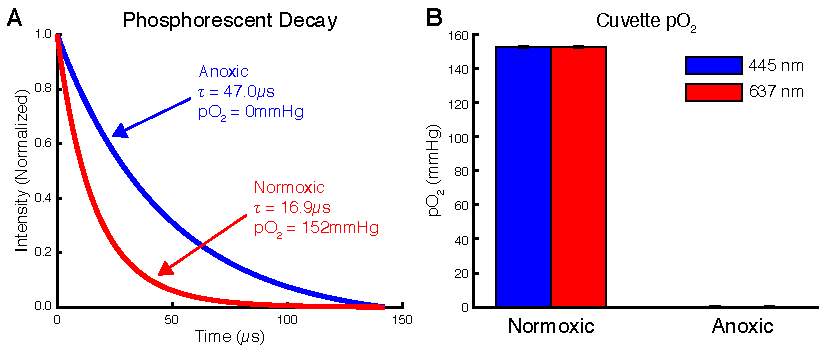
\includegraphics{figures/chapter_2/cuvette.pdf}
    \caption[Averaged phosphorescent decay curves in anoxic and normoxic cuvette environments with fitted lifetimes and their corresponding \ce{pO2} values.]{
        \label{fig:cuvette}
        \textbf{(A)} Averaged phosphorescent decay curves ($n$ = 200) in anoxic and normoxic cuvette environments with fitted lifetimes and their corresponding \ce{pO2} values. \textbf{(B)} Excitation wavelength does not affect measured \ce{pO2}. Adapted from \cite{Sullender:2018ff}.
    }
\end{figure}

%%%%%%%%%%%%%%%%%%%%%%%%%%%%%%%%%%%%%%%%%%%%%%%%%%%%%%%%%%%%%%%%%%%%%%%%%%%%%%%
\subsection{Fitted Lifetime Discrepancy}

The lifetimes of fluorescent and phosphorescent decays are independent of excitation wavelength. Targeting the Soret or Q band absorption maxima of a porphyrin should result in identical measurements of $\tau$ since internal conversion and vibrational relaxation occur on picosecond timescales. However, discrepancies in the phosphorescent decays were identified between 445 and 637 nm excitation (Figure \ref{fig:offsetcorrection}A). Fitting the exponential decays produced different values of $\tau$ from the same cuvette depending on the excitation. Since $\tau$ cannot vary with wavelength, this discrepancy likely arises because the two lasers are modulated using different mechanisms. The 445 nm laser is optically modulated using an AOM while the 637 nm laser is electronically modulated using its driver. Ideally both light sources should be modulated using the same technique to eliminate differences in bandwidth and modulation depth that can manifest in the optical signal.

In order to correct for this error, the exponential decay fitting process was modified with a temporal offset to ensure that both wavelengths would produce the same lifetime values. Figure \ref{fig:offsetcorrection}B depicts the relationship between the offset and the resulting fits for $\tau$ in the normoxic cuvette. As the offset is increased, the fitting is biased towards longer lifetimes. The optimal offsets were identified at $t$ = 21.50 $\mu$s for 445 nm excitation and $t$ = 26.54 $\mu$s for 637 nm excitation. These offsets result in a fitted $\tau$ = 16.993 $\mu$s (\ce{pO2} = 152 mmHg) and are used throughout this dissertation. A major disadvantage of this strategy is the waste of phosphorescent signal. In the normoxic cuvette, these offsets correspond to 96\% and 60\% of the peak phosphorescence intensity for 445 and 637 nm excitation, respectively. While the exact percentage scales with $\tau$, this can have detrimental effects on fitting performance for weak signals.

% Figure - Offset Correction
\begin{figure}
    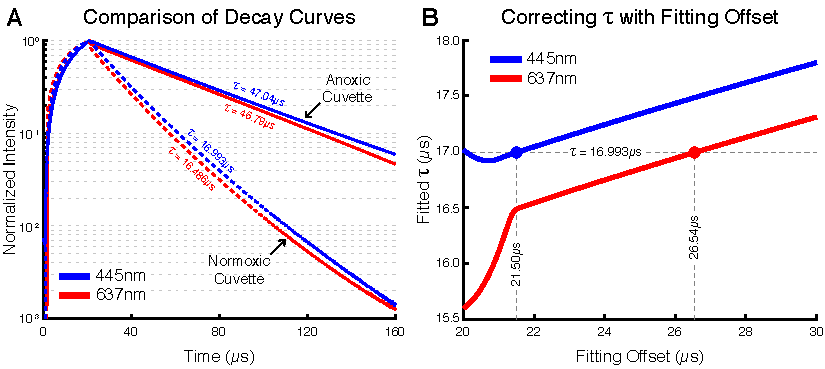
\includegraphics{figures/chapter_2/offsetcorrection.pdf}
    \caption{
        \label{fig:offsetcorrection}
        \textbf{(A)} 445 and 637 nm excitation produce different phosphorescent decay curves in identical samples. \textbf{(B)} Introducing an offset into the exponential decay fitting process corrects the wavelength-dependent lifetime discrepancy.
    }
\end{figure}

%%%%%%%%%%%%%%%%%%%%%%%%%%%%%%%%%%%%%%%%%%%%%%%%%%%%%%%%%%%%%%%%%%%%%%%%%%%%%%%
\subsection{Limitations of the Calibration Curve} \label{ssec:calibration_limit}

Performing measurements on the normoxic cuvette revealed a limitation of the Oxyphor PtG4 calibration curve (Figure \ref{fig:oxyphor_ptg4}B), which has a maximum \ce{pO2} of 160 mmHg. While this is well beyond normal physiological values, any measurements conducted in animal subjects receiving supplemental oxygen would require using the Stern-Volmer relationship to convert $\tau$ into \ce{pO2}. However, the calibration curve does not fit the Stern-Volmer relationship particularly well ($R^2$ = 0.9729) and results in a discontinuous transition between the two methods (Figure \ref{fig:sternvolmerfit}). Lifetime measurements shorter than 16.6 $\mu$s will abruptly drop from 160 to 134 mmHg. Because of this deviation from the expected kinetics, there is significant uncertainty in the true \ce{pO2} values beyond the range of the empirical data. Despite this limitation, the combination of the calibration curve and the fitted Stern-Volmer parameters are used throughout this dissertation. The calibration curve is used when 16.6 $\mu$s $\ge \tau$ $\ge$ 47 $\mu$s and the Stern-Volmer relationship is used when $\tau$ \textless{} 16.6 $\mu$s. When $\tau$ \textgreater{} 47 $\mu$s ($\tau_0$), \ce{pO2} is set to 0 mmHg.

% Figure - Stern-Volmer Fit
\begin{figure}
    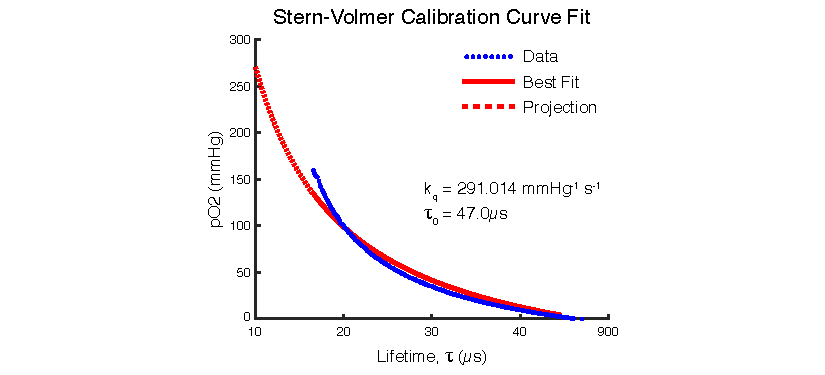
\includegraphics{figures/chapter_2/sternvolmerfit.pdf}
    \caption{
        \label{fig:sternvolmerfit}
        Least-squares fitting of the Stern-Volmer relationship to the Oxyphor PtG4 calibration data and the resulting prediction for lifetimes down to 10 $\mu$s. For $\tau > \tau_0$, \ce{pO2} is set to 0 mmHg.
    }
\end{figure}



%%%%%%%%%%%%%%%%%%%%%%%%%%%%%%%%%%%%%%%%%%%%%%%%%%%%%%%%%%%%%%%%%%%%%%%%%%%%%%%
% Section 2.3 - Demonstration of Acute In Vivo Imaging
%%%%%%%%%%%%%%%%%%%%%%%%%%%%%%%%%%%%%%%%%%%%%%%%%%%%%%%%%%%%%%%%%%%%%%%%%%%%%%%
\section{Demonstration of Acute \textit{In Vivo} Imaging}

The system was tested \textit{in vivo} using mice (CD-1, male, 25-30 g, Charles River) with permanent cranial window implants (see Appendix \ref{app:cranial_window}) that afford optical access to the surface of the brain. The window was positioned over the frontoparietal cortex approximately 2 mm rostral from bregma and 0.5 mm lateral from the sagittal suture. Animals with clear and healthy cranial windows were selected for use after at least two weeks of recovery post-surgery. The subject was anesthetized with medical air vaporized isoflurane (1.5\%) via nose-cone inhalation and placed supine in a head-fixed stereotaxic frame (Narishige Scientific Instrument Lab). Oxygen gas was intentionally avoided to prevent hyperoxia from interfering with the \ce{pO2} measurements. Vitals including oxygen saturation, heart rate, and breath rate were monitored via pulse oximetry (MouseOx, Starr Life Sciences) and temperature was regulated with a feedback heating pad (DC Temperature Controller, FHC). Oxyphor PtG4 was administered via retro-orbital injection into the venous sinus for a target blood plasma concentration of 5 $\mu$M. The subject was then placed under the dual-modality system for imaging.

% Figure - Static Speckle and ICT
\begin{figure}
    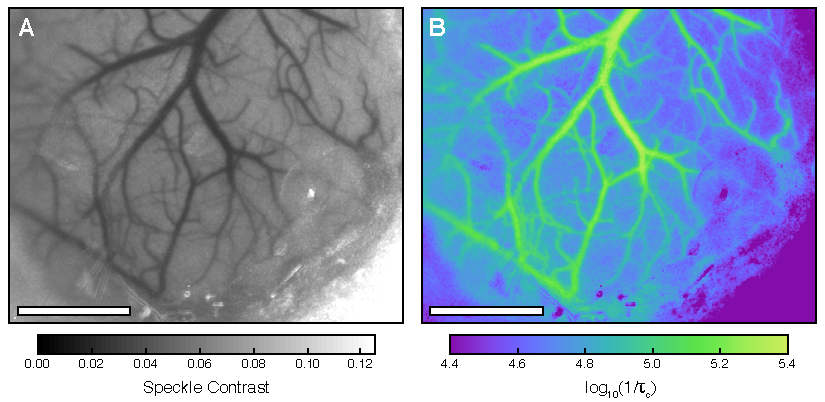
\includegraphics{figures/chapter_2/staticspeckle.pdf}
    \caption{
        \label{fig:staticspeckle}
        \textbf{(A)} Speckle contrast and \textbf{(B)} ICT images of the mouse cortex (Scale bars = 1 mm).
    }
\end{figure}

Figure \ref{fig:staticspeckle} depicts an averaged ($n$ = 45) speckle contrast image and its corresponding ICT image highlighting the vasculature of the cortex. Speckle contrast images in this document are displayed using a grayscale colormap spanning the full range of the speckle contrast histogram. ICT images are displayed on a logarithmic scale using a perceptually-balanced colormap \cite{Niccoli:vx} spanning the full range of the ICT histogram. Compared to the speckle contrast image, the ICT image more clearly depicts the flow profiles within the larger vessels.

Static oxygen tension measurements were acquired from two arterioles, two veins, and one parenchyma region using both the 445 and 637 nm excitation lasers (Figure \ref{fig:staticpO2}A). Patterns were displayed at 1 Hz for a total of 5 seconds with 2500 phosphorescent decays averaged per ROI. The measured \ce{pO2} within each region aligns well with physiological expectations with both arterioles exhibiting higher \ce{pO2} than the venous or parenchyma areas (Figure \ref{fig:staticpO2}B). The effects of wavelength can be seen as 445 nm excitation resulted in a broader range of \ce{pO2} values (48-83 mmHg) compared to 637 nm excitation (75-82 mmHg). Despite differences in absolute value, the trend of arterioles having greater \ce{pO2} than parenchyma, which in turn has greater \ce{pO2} than veins, exists for both excitation wavelengths. Since lifetime does not depend upon excitation wavelength (Figure \ref{fig:cuvette}B), these differences likely arise because of increased penetration depth at the longer wavelength.

% Figure - Static pO2
\begin{figure}
    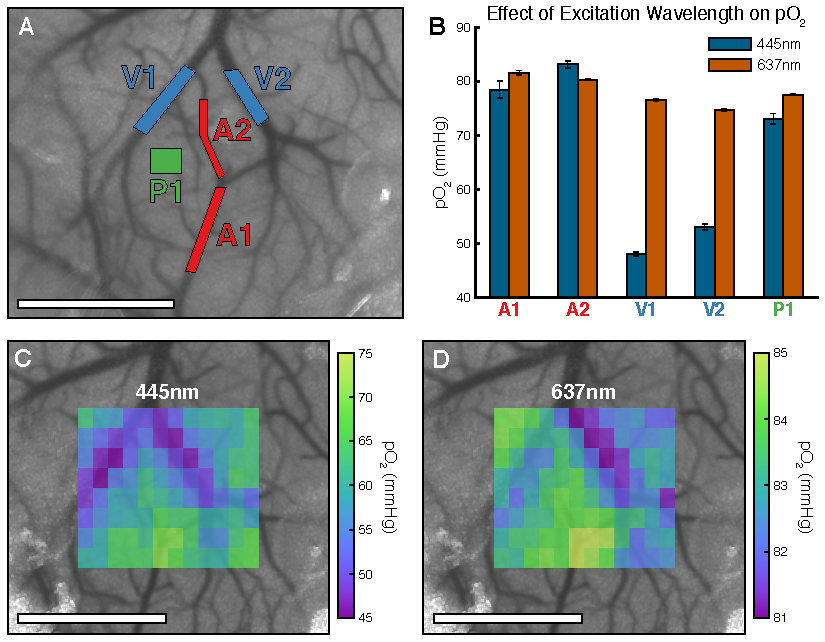
\includegraphics{figures/chapter_2/staticpO2.pdf}
    \caption[Static \textit{in vivo} measurements of cortical oxygen tension.]{
        \label{fig:staticpO2}
        \textbf{(A)} Speckle contrast image of cortical flow overlaid with regions targeted for \ce{pO2} measurements. Two descending arterioles (A1, A2), two veins (V1, V2), and one parenchyma region (P1) were examined. The projected patterns ranged between 0.014 - 0.046 mm$^2$ in area. \textbf{(B)} \ce{pO2} measurements within the targeted regions conducted using both 445 and 637 nm excitation of Oxyphor PtG4 (mean $\pm$ s.d.). \textbf{(C)} 445 nm and (d) 637 nm \ce{pO2} maps produced using tiled excitation patterns covering a 1.2 x 1.0 mm area. Each individual tile has a projected area of 0.012 mm$^2$ (Scale bars = 1 mm). Adapted from \cite{Sullender:2018ff}.
    }
\end{figure}

In order to obtain a more comprehensive look at vascular oxygenation within the camera FOV, an array of 12 x 8 rectangular tiles was sequentially projected using the DMD. The tiles were displayed at 10 Hz with 250 decays averaged per pattern for a total acquisition time of 9.6 seconds. The resulting \ce{pO2} maps (Figure \ref{fig:staticpO2}C-D) coarsely follow the visible surface vasculature. As expected, the large branching vein has lower \ce{pO2} values compared to the arteriole approaching from the bottom of the FOV or the surrounding parenchyma. 445 nm excitation again resulted in a wider range of \ce{pO2} values (45-85 mmHg) compared to 637 nm excitation (81-85 mmHg).

%%%%%%%%%%%%%%%%%%%%%%%%%%%%%%%%%%%%%%%%%%%%%%%%%%%%%%%%%%%%%%%%%%%%%%%%%%%%%%%
\subsection{Hyperoxic Challenge}

The ability to detect changes in cortical oxygen tension was tested using an hyperoxic challenge. The oxygen fraction of inspired air under anesthesia was increased from 21\% (normoxia) to 100\% and then decreased back to normoxia for recovery. Hyperoxia was maintained for five minutes and \ce{pO2} measurements using 445 nm excitation were acquired at the end of each stage from three regions covering an arteriole, venule, and parenchyma (Figure \ref{fig:hyperoxicchallenge}A). The patterns were displayed at 1 Hz with 2500 phosphorescent decays averaged per ROI. A large increase in \ce{pO2} was detected during the hyperoxic state across all three regions (Figure \ref{fig:hyperoxicchallenge}B) with the arteriole experiencing the largest net increase (+120 mmHg). The \ce{pO2} remained slightly elevated above baseline values several minutes later during the post-hyperoxia recovery stage.

The measured lifetime in the arteriole during hyperoxia was only 13.1 $\mu$s and therefore exceeds the limits of the Oxyphor PtG4 calibration curve (Section \ref{ssec:calibration_limit}). The Stern-Volmer relationship was used to calculate the \ce{pO2} and likely underestimates the actual value. While it is counterintuitive for the arteriole to experience the largest increase in \ce{pO2}, similar results were seen during hyperoxic retinal imaging in both mice and rats \cite{Shonat:2003ia}.

% Figure - Hyperoxic Challenge
\begin{figure}
    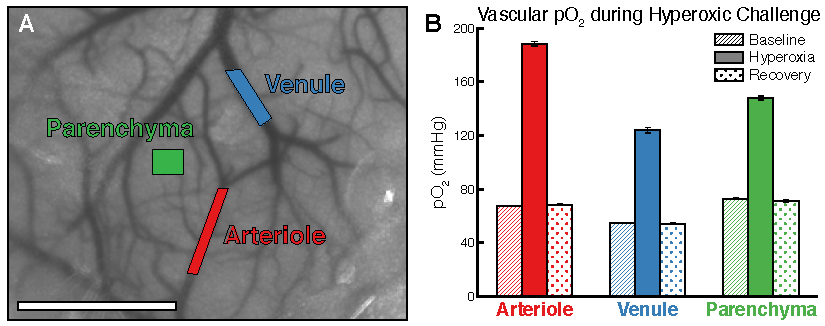
\includegraphics{figures/chapter_2/hyperoxicchallenge.pdf}
    \caption[\ce{pO2} measurements from an ateriole, venule, and parenchyma during an hyperoxic challenge.]{
        \label{fig:hyperoxicchallenge}
        \textbf{(A)} Speckle contrast image depicting three regions (arteriole, venule, and parenchyma) targeted for 445 nm \ce{pO2} measurements during an hyperoxic challenge. \textbf{(B)} Static \ce{pO2} during baseline, hyperoxic, and recovery stages for each of the targeted vessels (mean $\pm$ s.d.). (Scale bar = 1 mm). Adapted from \cite{Sullender:2018ff}.
    }
\end{figure}

%%%%%%%%%%%%%%%%%%%%%%%%%%%%%%%%%%%%%%%%%%%%%%%%%%%%%%%%%%%%%%%%%%%%%%%%%%%%%%%
\subsection{Effects of Excitation Wavelength on Measured \ce{pO2}}

The results in Figure \ref{fig:staticpO2} revealed major differences in measured \ce{pO2} depending on excitation wavelength. The static \ce{pO2} measurements under 445 nm illumination spanned a range five times larger than that of 637 nm illumination. This discrepancy was most noticeable in venous regions, with the shorter excitation wavelength resulting in \ce{pO2} values around 50 mmHg whereas the longer wavelength resulted in values around 75 mmHg. Since depth penetration is heavily dependent upon wavelength \cite{Deng:2003kb}, the difference is likely the result of photons sampling a much larger volume of tissue during 637 nm illumination.

An estimate of transmission through a surface vessel at both wavelengths can be obtained using the Beer-Lambert Law. Because scattering increases the distance traveled by photons in tissue, this represents the most conservative estimate of the effect of wavelength on transmission. Assuming hemoglobin is the primary absorber in blood plasma with a concentration of 2.3 mM\cite{Robles:2010cw} and 95\% SaO2, the transmittance at 445 nm and 637 nm through a 100 μm arteriole is 0.9\% and 96.5\%, respectively. As excitation wavelength approaches the tissue optical window, the transmission of incident light significantly increases. The 445 nm light is almost entirely confined within a vessel of that caliber and does not extensively sample deeper microvasculature. Because the 637 nm light penetrates further into the brain, the measured pO2 is skewed away from the vascular value and is more representative of a bulk volumetric average. This is consistent with prior Monte Carlo modeling that found fluorescence primarily originates from within large surface vasculature at shorter wavelengths \cite{Davis:2011wj}. As excitation wavelength increases, a larger fraction of the detected fluorescence originates from beyond the vessel.

These results indicate that excitation wavelength must be considered when performing single-photon fluorescent or phosphorescent measurements using dyes with multiple excitation maxima. Longer wavelengths would not be ideal for studying surface vasculature because of the increased penetration depth but would be better suited for examining parenchyma regions or bulk areas. Conversely, the limited penetration depth of shorter excitation wavelengths, especially in vasculature, make them ideal for restricting measurements to only surface tissue.



%%%%%%%%%%%%%%%%%%%%%%%%%%%%%%%%%%%%%%%%%%%%%%%%%%%%%%%%%%%%%%%%%%%%%%%%%%%%%%%
% Section 2.4 - Discussion
%%%%%%%%%%%%%%%%%%%%%%%%%%%%%%%%%%%%%%%%%%%%%%%%%%%%%%%%%%%%%%%%%%%%%%%%%%%%%%%
\section{Discussion}

The dual-modality imaging system combining LSCI and oxygen-dependent quenching of phosphorescence is a purely optical, non-contact platform for measuring CBF and \ce{pO2}. The system builds upon prior work by Ponticorvo and Dunn \cite{Ponticorvo:2010uv} by using structured illumination to overcome the traditional limitations of lifetime imaging. Spatially patterning excitation light with a DMD allows for the use of a point detector, which offers both high sensitivity and speed for the collection of the phosphorescent signal. Ultimately, the spatial and temporal resolutions of the phosphorescent measurements are limited by noise. Regions as small as 0.01 mm$^2$ could reliably be excited at a pattern repetition rate of 10 Hz with 250 phosphorescent decay curves accumulated per ROI. Because intensity of the excitation light scales with the number of DMD pixels in the ON state, larger patterns could allow for even faster pattern rates at the expense of averaging (e.g. 100 Hz with 25 decays averaged per ROI). However, a 10 Hz pattern rate is more than sufficient for visualizing many dynamic physiological events in the brain.



%%%%%%%%%%%%%%%%%%%%%%%%%%%%%%%%%%%%%%%%%%%%%%%%%%%%%%%%%%%%%%%%%%%%%%%%%%%%%%%
% END Chapter 2
%%%%%%%%%%%%%%%%%%%%%%%%%%%%%%%%%%%%%%%%%%%%%%%%%%%%%%%%%%%%%%%%%%%%%%%%%%%%%%%
